\documentclass{article}
\usepackage{apamposter}
\usepackage[square,numbers]{natbib}
\usepackage{lmodern}
\usepackage{textpos}
\setcounter{secnumdepth}{2}
\newcommand{\nb}[1] {\textcolor{red}{#1}}
\setlength{\TPHorizModule}{1in}
\setlength{\TPVertModule}{1in}
\begin{document}
\bibliographystyle{plainnat}
%\begin{center}
%

% Start of title...

%

% switch into sans-serif for title

\begin{textblock}{70}(0,0)

\textblockcolor{white}

\begin{center}

\vspace{5mm}\def\myfig#1{\begin{center}\includegraphics[width=\graphicswidth]{#1}\end{center}}

{\veryHuge\color{black} \textbf{Design, Fabrication, Installation and First Results of the HBT-EP Shaping Coil}}

\vspace{15mm}

\LARGE\textbf{\color{lnavy}
P. Byrne$^\dagger$, J. P. Levesque, D. Rhodes, Q. Peng, G. Navratil, M. E. Mauel \hspace{2in} \emph{Columbia University}}\\

\vspace{5mm}

\end{center}
\end{textblock}
\begin{textblock}{12}(55,3)
\begin{flushright}

\hspace{950mm}{$^*$Supported by U.~S.~DOE Grant DE-FG02-86ER53222. }\hspace{1in}\\
\hspace{950mm}{\color{black}$^{\dagger}$email: {pjb2132@columbia.edu} }\hspace{1in}

\end{flushright}
\end{textblock}

\begin{textblock}{3}(.2,.6)


\includegraphics[scale =.75]{CU_logo_exported.png}

\end{textblock}


\begin{textblock}{1}(65,.45)


\includegraphics[scale =1]{hbt_logo.png}

\end{textblock}

\vspace{120mm}


% End of title, start of content..

%\fbox{\parbox[b][4em][t]{0.33\textwidth}{Some \\ text} }
%\fbox{\parbox[c][4em][s]{0.33\textwidth}{Some \vfill text} }
%\fbox{\parbox[t][4em][c]{0.33\textwidth}{Some \\ text} }

%\begin{minipage}[b][5\baselineskip][b]{3in}
  %%\centering
  %%\vspace{.25in}
  %%\begin{flushleft}
  %
\includegraphics[width=3in]{CU_logo_exported.png}
  %%\end{flushleft}
%\end{minipage}
%\begin{minipage}[t][5\baselineskip][t]{.75\textwidth}
    %\centering
    %\VeryHuge{\textbf{
%Design, Fabrication, Installation and First Results of the HBT-EP Shaping Coil}}\\
    %\vspace{.25in}
    %\Huge{\textbf{\color{lnavy}
%P. Byrne, J. P. Levesque, D. Rhodes, Q. Peng, G. Navratil, M. E. Mauel \hspace{2in} Columbia University}}
%\end{minipage}
%\begin{minipage}[b][5\baselineskip][b]{3in}
  %\begin{flushright}
  %\vspace{.25in}
  %
\includegraphics[width=3in]{hbt_logo.png}
  %\end{flushright}
%\end{minipage}
%%\includegraphics{leftlogo}\hfill Text\hfill\includegraphics{rightlogo}
%%\VeryHuge{\textbf{
%%Design, Fabrication, Installation and First Results \\
%%of the HBT-EP Shaping Coil}}\\
%%\vspace{.25in}
%%\Huge{\textbf{
%%P. Byrne, J. P. Levesque, D. Rhodes, Q. Peng, G. Navratil, M. E. Mauel \hspace{3in} Columbia University}}
%%\end{center}
%%\begin{flushright}
%%
\includegraphics[width=0.075\columnwidth]{hbt_logo.png}
%%\end{flushright}
%\vspace{.25in}
%%\end{VeryHuge}
\begin{multicols}{5}
\section{Abstract}

%\begin{itemize}
A low self-and-mutual inductance, zero net turn coil and its capacitive power supply have been fabricated and installed on the HBTEP Tokamak.  The coil is used to locally shape HBT-EP's normal circular cross section, up to and including the creation of a poloidal field null above the inboard midplane.  This will enable HBT-EPs first investigation of the effects of shaping on the MHD multimode spectrum.  Post installation tests have affirmatively proven the ability of the coil to impose a continuum of shaping, from circular to fully diverted. A description of the coil system, it's components, and qualifying tests are below.  Results of initial experiments with are also provided and compared with simulations.\\

 HBT-EP is passively stabilized against n=0 positional instabilities

%\end{itemize}

\section{Design and Fabrication}
\subsection{The Coil}
\begin{itemize}
\item The HBT-EP shaping coil provides up to 40kA-turns of current.  HBT-EP's usual I$_{\mbox{plasma}}$ is ~10-15kA
\item The coil consists of a single 1$/$0 welding wire, wound toroidally 8 times. It is located slightly above the high field side midplane.
\item The 8 loops are distributed into 3 bundles, consisting of 2, 4, and 2 windings.
\item The winding reverses direction twice, such that the central 4-loop bundle is carries current in to opposite direction from the flanking 2-loop bundles.\\
\begin{center}
\vspace{.25in}
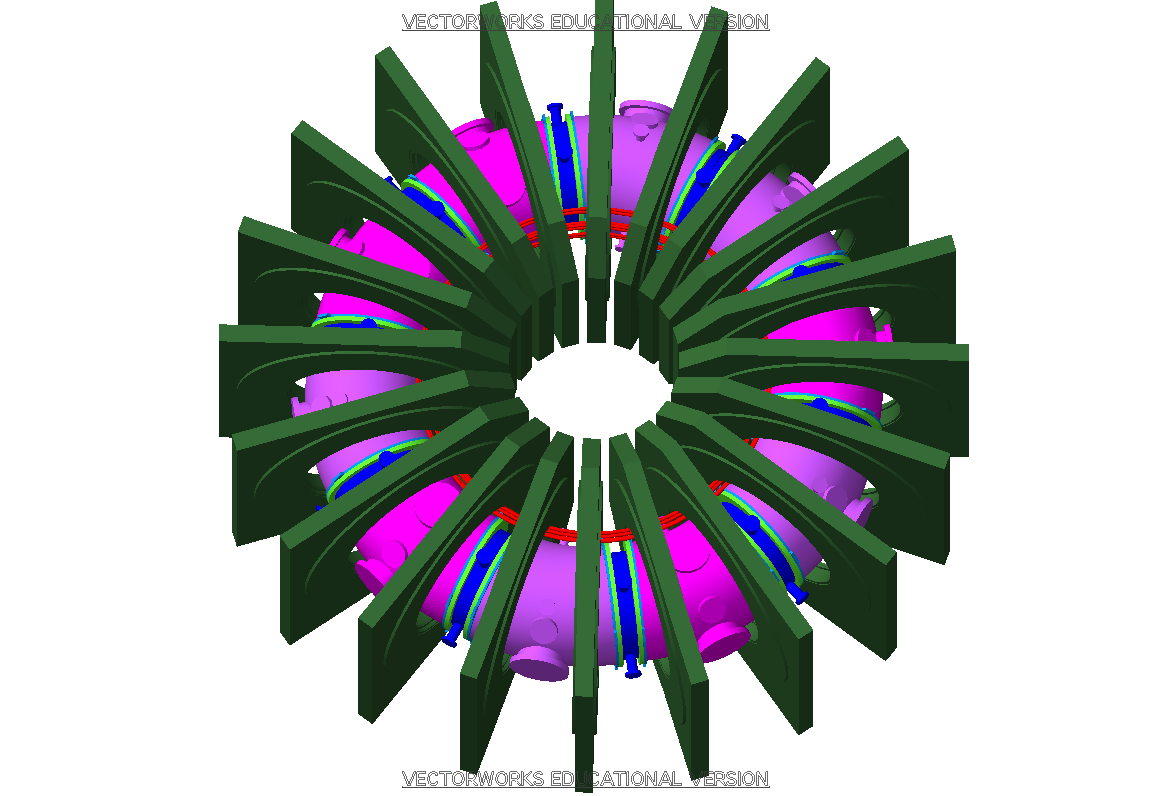
\includegraphics[width=0.9\columnwidth]{HBT-EP_Full2.pdf}\\
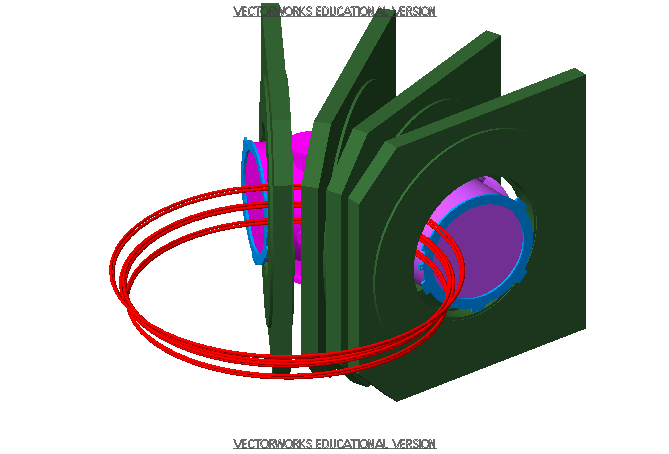
\includegraphics[width=0.9\columnwidth]{HBT-EP_Section.pdf}
\newline
Fig. 1\\
Full and sectioned views of the HBT-EP Tokamak\\
with the new shaping coil installed\\
\vspace{.25in}
\end{center}
\item Zero-Net-Turns constrution keeps coil self and mutual inductance low, and the shaping of the plasma extremely localized to a few poloidal degrees from the location of the coil.
\item The coil's low inductance (42$\mu$H) and low resistance($<$50m$\Omega$) allow for the use of a low energy, low voltage power supply.
\subsection{The Power Supply}
\begin{center}
\vspace{.25in}
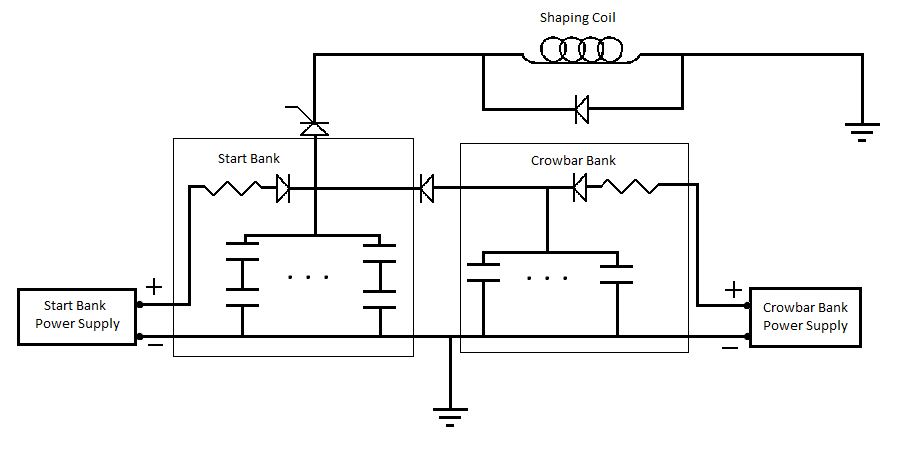
\includegraphics[width=0.9\columnwidth]{Simplified_bank_diagram.png}
\newline
Fig. 2\\
Diagram of the HBT-EP shaping circuit.\\
Start bank is high voltage, fast risetime.\\
Crowbar bank is low voltage, high capacitance.\\
\vspace{.25in}
\end{center}
\item The shaping fields are sustained by capacitive discharge, provided by a 900V, 7.5mF startup bank, and a 250V, 0.6F crowbar bank.  
\item The capacitors are fired in two-stages, the start bank providing a quick establishment (850$\mu$s) and the crowbar bank long sustainment (90$\%$ of max current after 6ms) of the shaping field.
\item The power supply provides up to 40kA-turns of shaping current with only 22kJ of energy thanks to impedance minimizing design.
\item The crowbar bank is soft-switched into the circuit passively using a high current rectifier, ensuring a smooth transition from start-up to steady-state regimes\\
\vspace{.25in}
\begin{center}
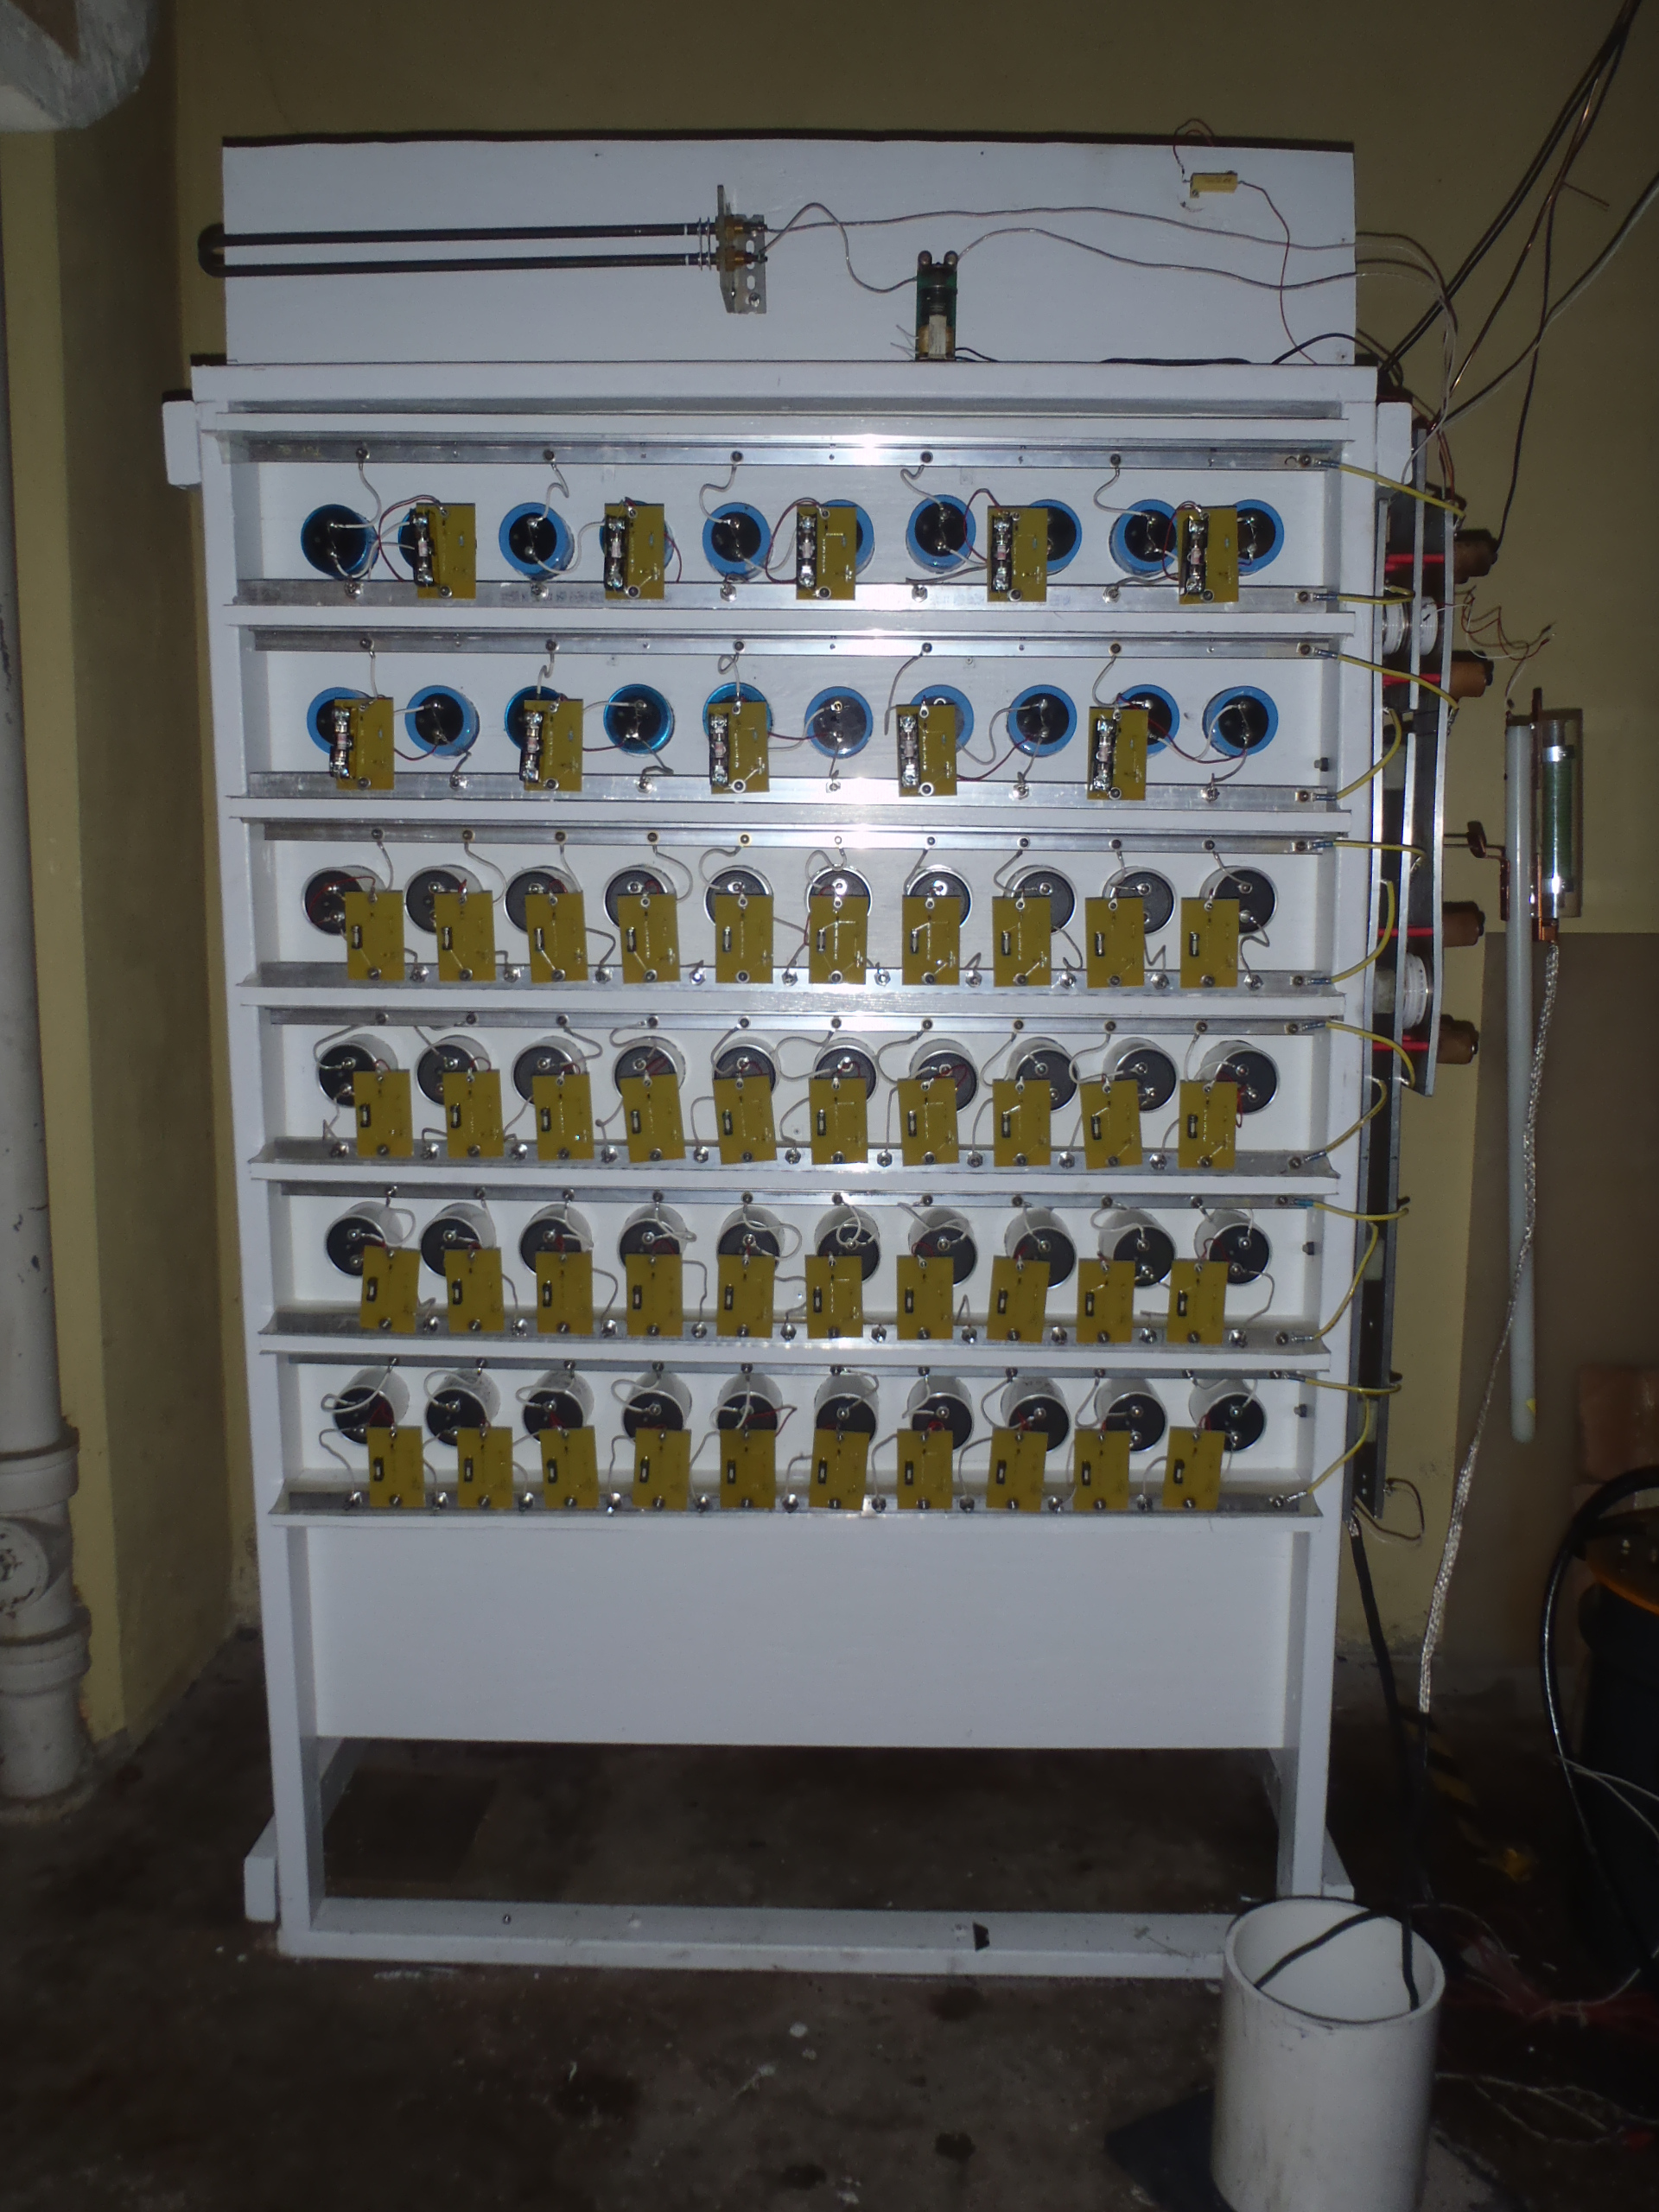
\includegraphics[width=0.9\columnwidth]{Cap_bank.jpg}\\
Fig. 3\\
The HBT-EP shaping power supply\\
Start bank caps are blue, crowbar bank caps are white\\
Low required operating energy allows for compact construction\\
\vspace{.25in}
\end{center}
\section{Operation and Qualification}
\item Pulse amplitude and shape are controlled by selecting voltages on each bank; allowing for slower startup, tracking of shaping current to plasma current and/or position, and degree of plasma shaping - up to and including a fully diverted discharge.
\item Voltages and capacitances selected in design phase via SPICE simulations to allow a maximum shaping current of ~9kA/turn\\
\vspace{.25in}
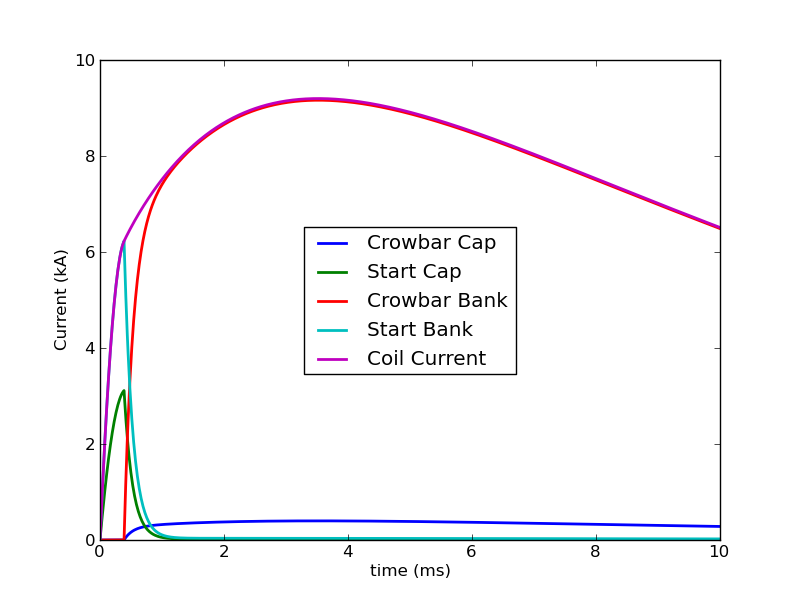
\includegraphics[width=0.9\columnwidth]{bank_currents.png}
\begin{center}
Fig. 4\\
SPICE simulation of cap bank discharge at maximum voltage\\
Passive switching allows smooth transition to crowbarred operation\\
\end{center}
\vspace{.25in}
\item Shaping current is monitored by means of a rogowski coil manufactured in-house.
\item Comparison of simulated pulse traces to actual operation shows higher current than expected.
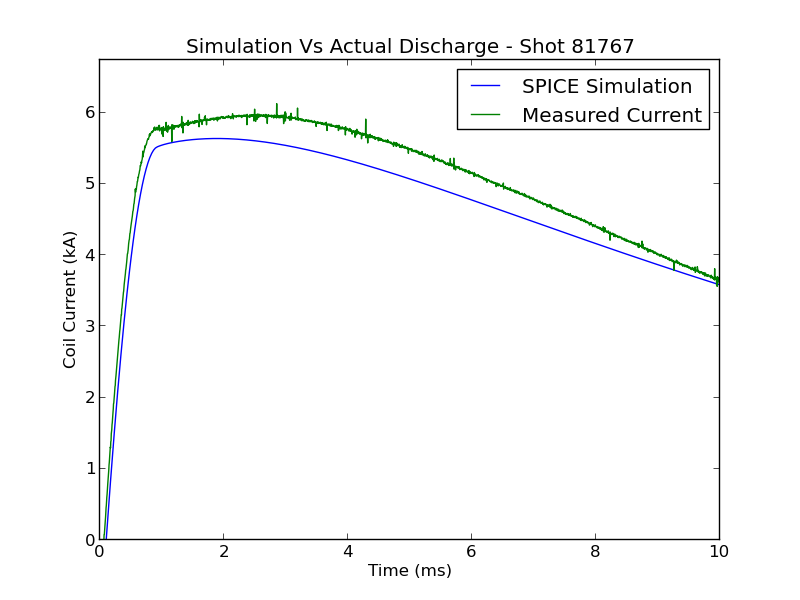
\includegraphics[width=0.9\columnwidth]{shaping_current_sim_vs_real_81797.png}
\begin{center}
Fig. 5\\
SPICE simulation of standard discharge\\
compared to current as meaured in the coil\\
\end{center}
\item Design points of coil were 49$\mu$H, 22m$\Omega$. Inductance measured @ 42 $\mu$H, resistance is too low to measure, but 17-18m$\Omega$ can be inferred from pulse shape.
\item HBT-EP plasmas have been run diverted using ~70$\%$ of available current
\item Modeling of flux surfaces using filamentary currents suggests HBT-EP has been successfully run diverted.\\
\vspace{.25in}
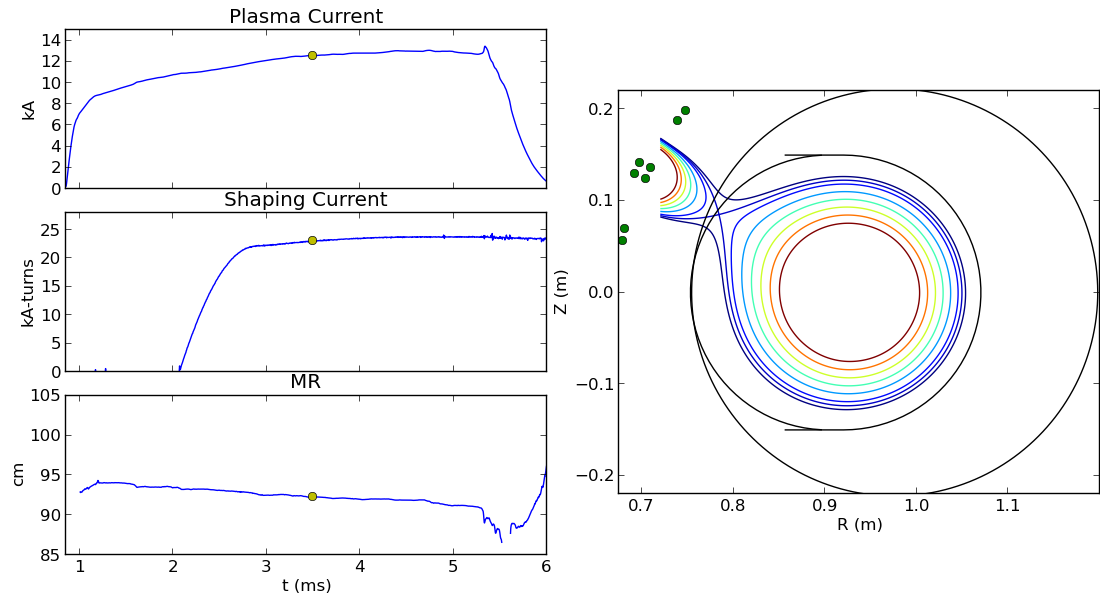
\includegraphics[width=0.9\columnwidth]{flux_surfaces_during_shaping.png}
\begin{center}
Fig. 6\\
Flux Surface reconstruction using data from HBT-EP shot 81597\\
Green dots represent physical location of shping coil turns.\\
Black lines represent vacuum chamber and plasma limiting surfaces\\
\end{center}
\vspace{.25in}
\item Toroidal non-axisymmetries are present due to pre-existing diagnostics impeding the run.
\item The largest non-axisymmetry has been modeled and shown to have the effect of increasing the coupling of the coil to the plasma\\
\vspace{.25in}
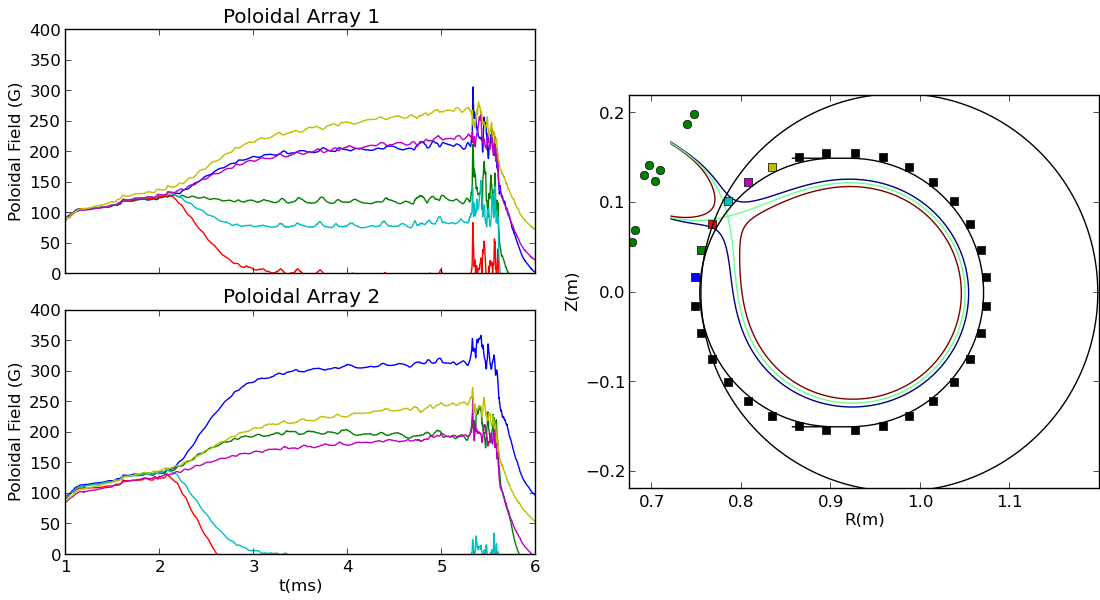
\includegraphics[width=0.9\columnwidth]{poloidal_field_cancellation_APS_2013.png}
\begin{center}
Fig. 7\\
Poloidal field measured at two toroidal locations near HBT-EP x-point for shot 81597.\\
$B_p$ traces are color coded to the sensors as shown on the right.\\
$B_p$ has a zero crossing at both locations, but is stronger in one than another\\
\end{center}
\item The plasma is still diverted, but will have a larger scrape-off layer than otherwise
\item Plasmas being shaped are more susceptible to diversion, but shots have been taken with steady MR, that are not extreme outboard.
\item Study of decay index last year showed that we should be able to develop a stable shot.
\item Mode analysis is so far inconclusive, as the spectra of diverted shots do not seem significantly different from limited ones
\item future work: develop a longer lived diverted discharge
\item future work: increase the database of diverted plasmas
\item future work: search the database for or develop an unshaped shot with similar parameters (MR,IP,q*) for a direct comparison to diverted discharges
\item future work: work to understand, and if possible, mitigate the toroidal asymmetries in the coil
\item plots to display:
\item updated model of HBT-EP
\item flux surfaces during shaping - show diversion
\item MR (and IP ?) trace for a 'hard crash' shaped shot
\item comparison of simulation of bfields tree data at TA
\item comparison of simulation of bfields tree data at PA
\item stripey plot of shaped q=3 shot: best of 81593-98 compared to stripey plot of unshaped q=3 shot
\item BD dominant modes and spatial structures from shaped to unshaped


\end{itemize}

\section{Shaping Physics}

\begin{itemize}
\item Simulations of shaped and unshaped plasmas using TokaMac and DCON show change in expected resonant plasma modes
\item MHD multimode response shows reduction of multimode effects with shaping.\\

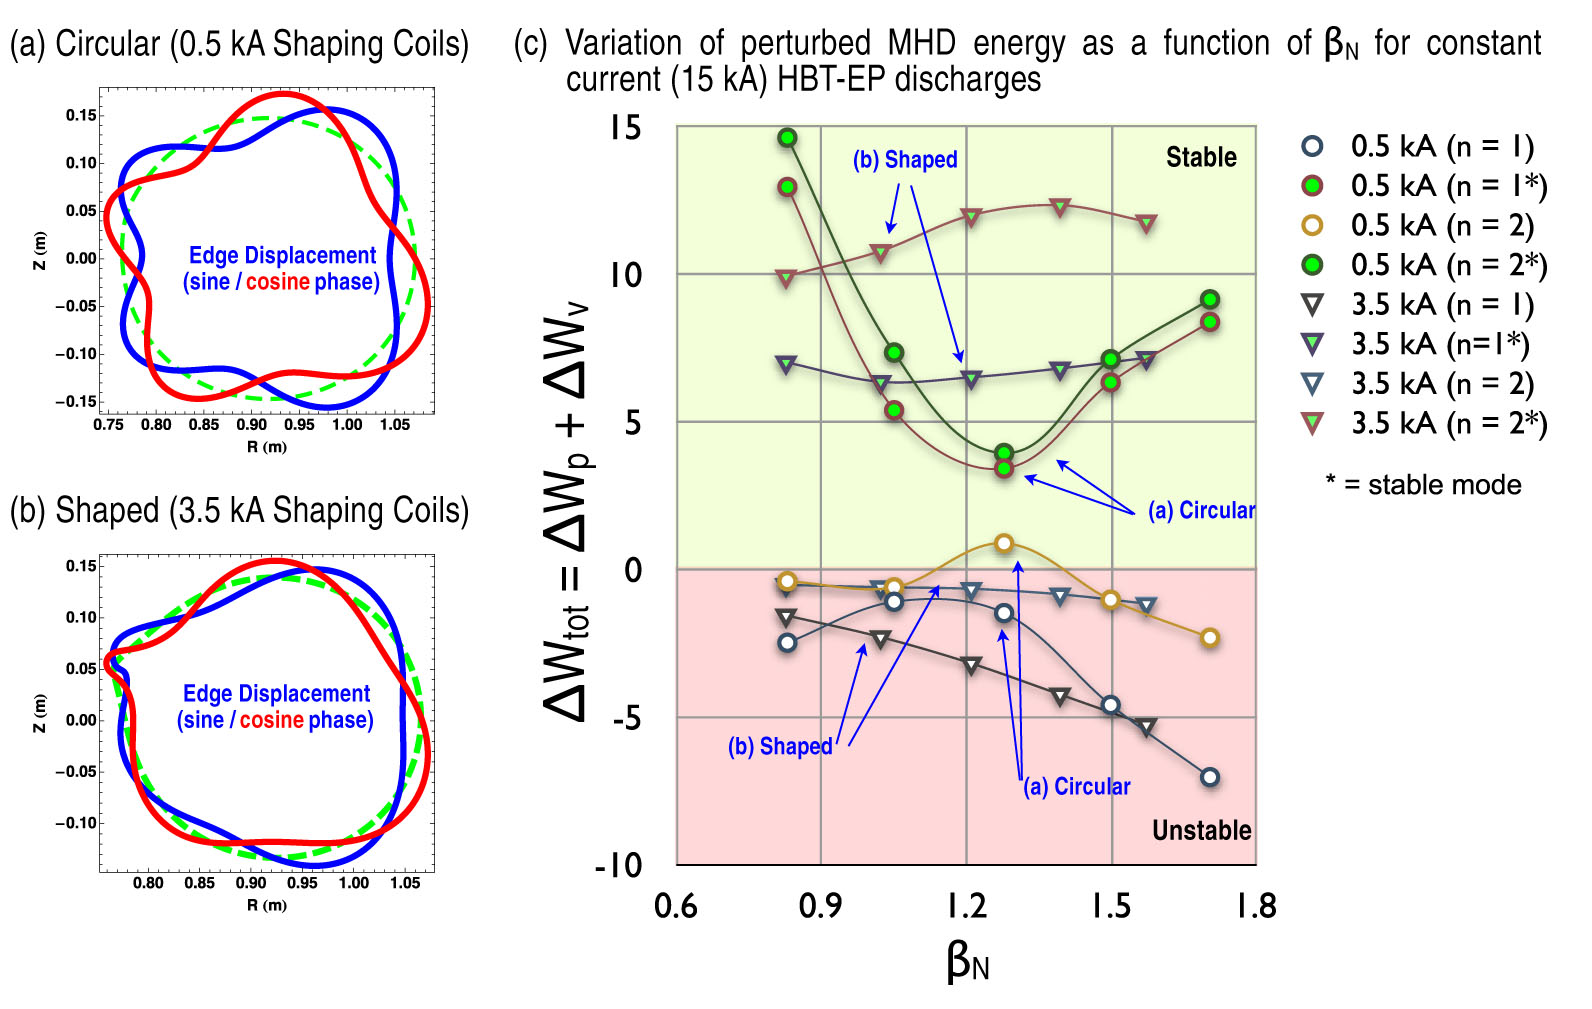
\includegraphics[width=0.9\columnwidth]{ModeDWimage2}


\item Unstable and ``most marginal" modes are observed for n = 1 and n = 2 in circular and shaped plasmas. 
\item There is a strong multimode response across all modes for the unshaped plasma when  $\beta$$_n$ rises past 1.2 (correlates to q$_a$=3).  Beta was scanned by taking a typical HBT-EP plasma equilibria and varying the core pressure$^{[1]}$

%\begin{center}Calculation of MHD multimode response for shaped and unshaped plasma.\\
%4 modes are observed for circular and shaped plasmas, the unstable mode \\
%and the "most marginal" modes for the cases n = 1 and n = 2. There is a \\
%strong multimode response across all modes for the unshaped plasma when \\
%$\beta$$_n$ rises past 1.2 (correlates to q$_a$=3).  Beta was scanned by taking a typical \\
%HBT-EP plasma equilibria and varying the core pressure\end{center}

\end{itemize}

\section{Simulations}

\section*{Coil-Plasma Coupling}

\begin{itemize}
\item Need to optimize coil geometry for low current demands, and low bulk plasma shape distortion.  
\item Widening the counterwound bundle spacing lowers the necessary current, but increases plasma shape distortion and coupling to machine magnetics.\\
\end{itemize}

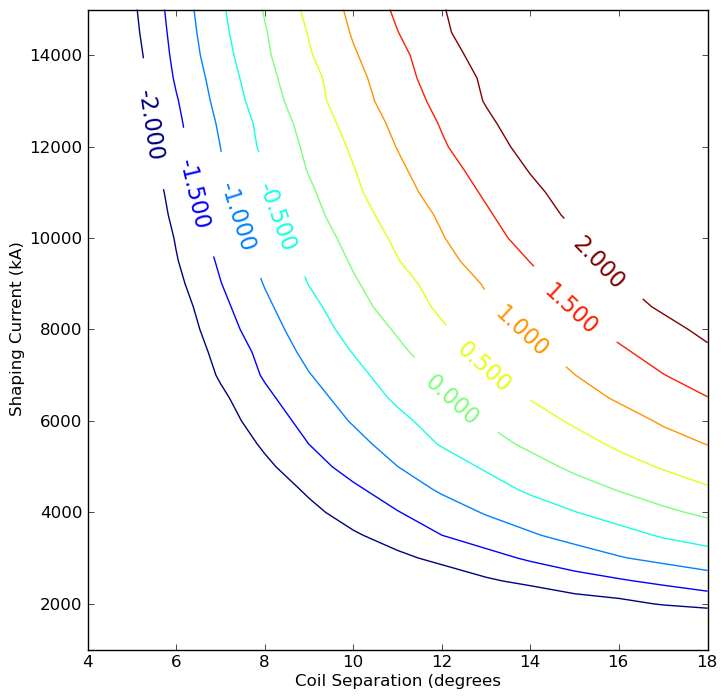
\includegraphics[width=0.9\columnwidth]{diversion_currents}

\begin{center}Contour plot of separatrix distance from inboard limiter\\ Positive numbers represent distance in centimeters into the plasma.\\Coil designed point: 10 degrees separation with 10kA peak current supply\\\end{center}

\section*{Positional Stability}
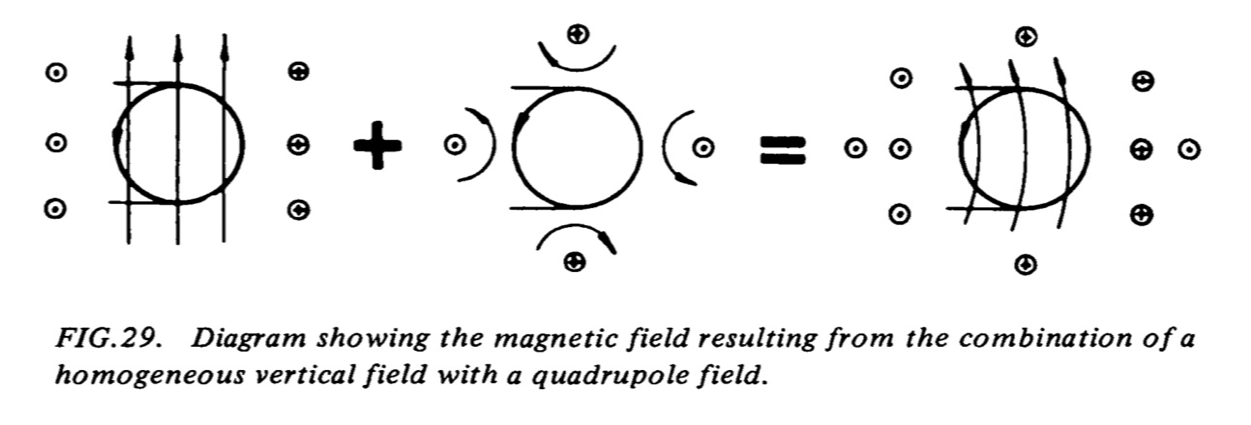
\includegraphics[width =0.9\columnwidth]{vacuumfield}\\
\begin{itemize}
\item Tokamak vacuum fields must include a vertical field as well as a dipole field
\item This field geometry imposes restoring forces on the plasma current for vertical or horizontal displacements.
\item The measure of positional stability is the decay index, n defined as:
\begin{center}
n $\equiv$ - $\frac{R}{B_z}$ $\frac{dB_Z}{dR}$
\end{center}
with stability is defined as:

\begin{center}
0 $\le$ n $\le$ 1.5
\end{center}

with negative n corresponding to vertical instabilities, and n \textgreater  1.5 corresponding to an inward instability.

\item Stronger Vertical Field (VF) Coil currents provide a more strongly stabilizing vacuum field
\item Typical currents are $\approx$ 2kA, or 10 \% of destabilizing Ohmic Heating (OH) coils

\includegraphics[width =0.45\columnwidth]{stability_space_tight}\includegraphics[width =0.45\columnwidth]{stability_space_shaped_tight}
\begin {center}
In a shaped plasma, the transition from stable to unstable occurs simultaneously across a large area and the necessary stabilizing current is larger. (Plasma centered @ 92cm)\\

\end{center}

\item HBT-EP is designed with positional stability maintained throught plasma lifetime on a standard shot.
\item Database review of nonstandard high OH, Low VF shots show slow growth rates for positional instabilities
\item Plasma tends to fall inwards when stability is lost, but typically survives for $\approx$ 2ms (or 20\% of normal lifetime) after losing stability.  
\item Slow growth rate will allow HBT-EP enough time to study the plasma's MHD behavior before any vacuum-field related instabilities cause it to disrupt.\\

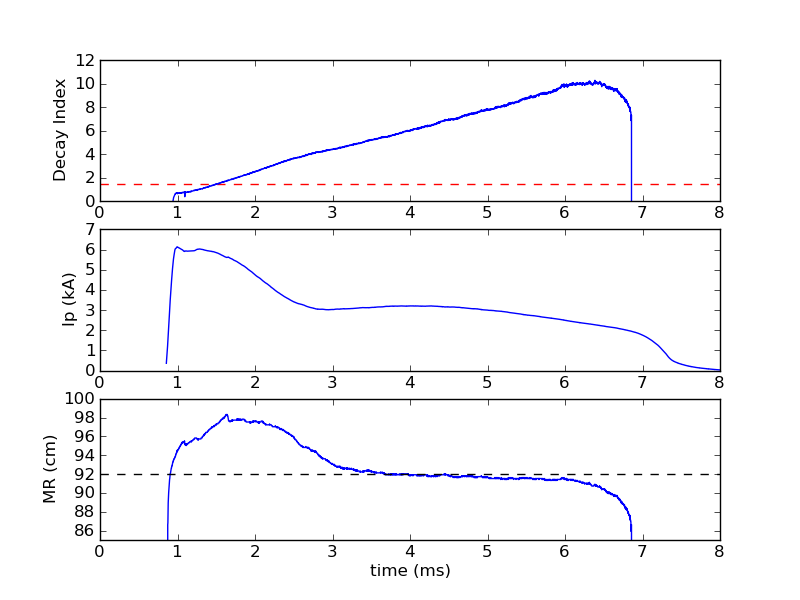
\includegraphics[width =0.9\columnwidth]{unstable_plasma}


\begin{center}
Plasma surviving positional instability (n$\gg$1.5) for nearly 6ms\\
Plasma remains stable in the center of the chamber (92cm) for nearly 3ms.\\
\end{center}
\end{itemize}

\section*{Capacitive Power Supply}

\begin{itemize}

\item Low C/High V start bank drives sharp current ramp; discharges in 0.5 ms.
\item High C/Low V crowbar bank is passively switched into the circuit as blocking diodes conduct
\item SPICE simulations predict system is overdamped; electrolytic caps safe from reverse biasing
\item Bank voltages can be tailored to shape the pulse, keeping separatrix position constant during discharge.\\
\begin{center}
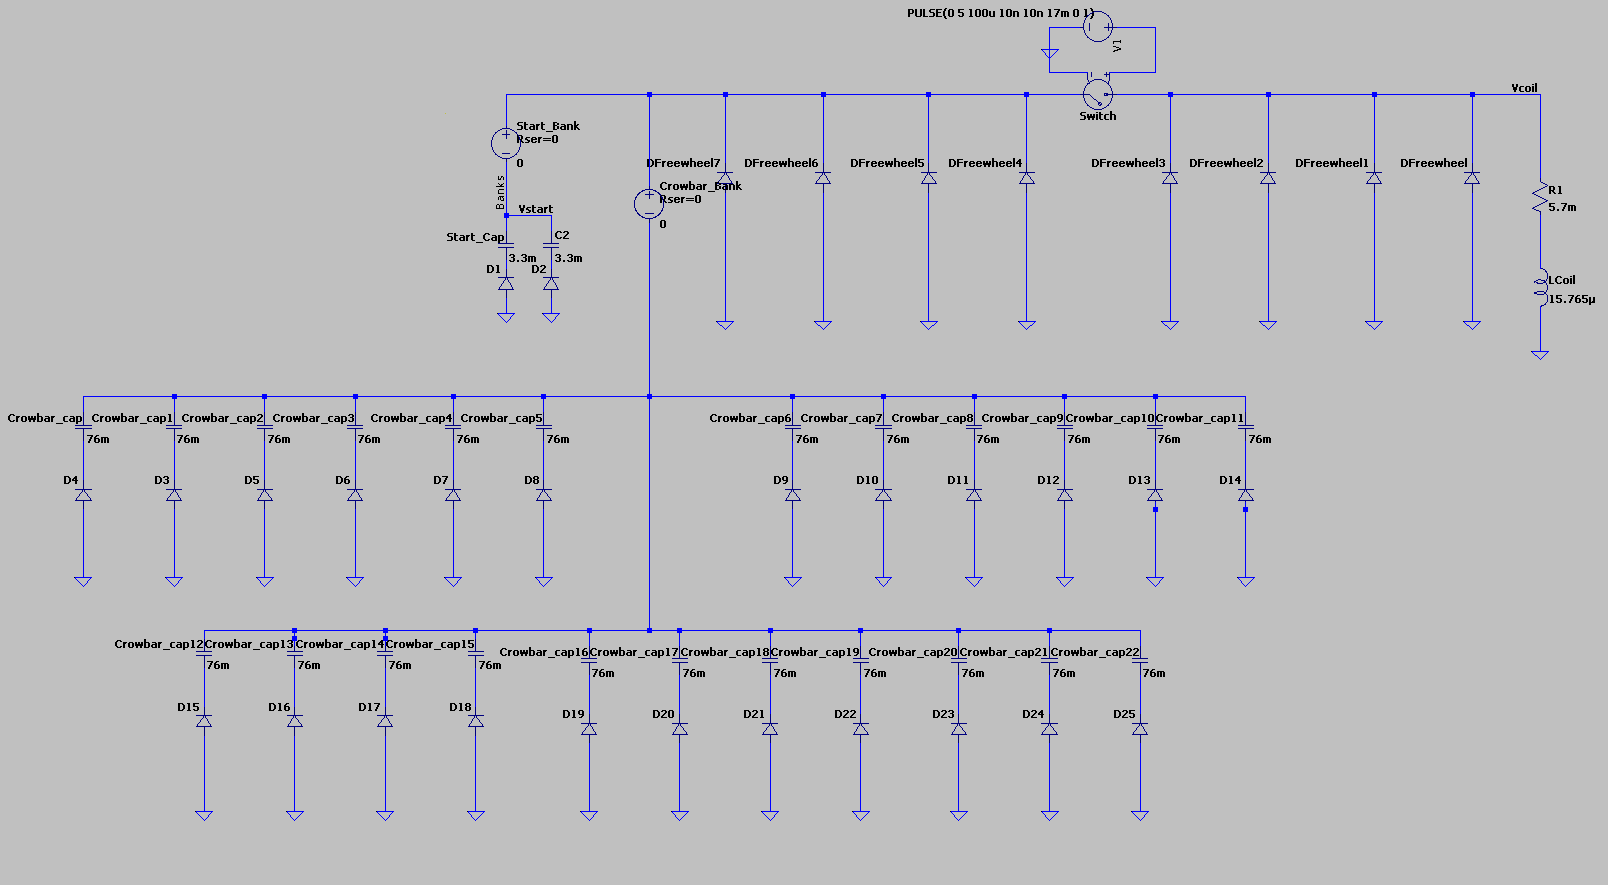
\includegraphics[width=.9\columnwidth]{Picture_7}

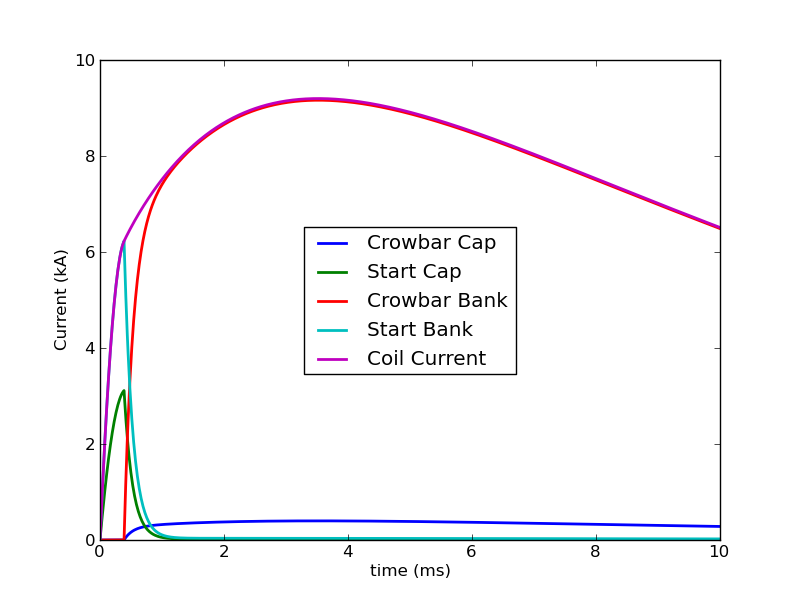
\includegraphics[width=0.9\columnwidth]{bank_currents}
SPICE simulation of cap bank discharge.\\
Passive switching allows smooth transition to crowbarred operation.\\
Current reaches maximum after 2ms, and spends roughly 2ms above 9kA\\
Time to onset and duration of diversion adjustable through bank settings
\end{center}

\end{itemize}

\section{Control Coil Shaping}
\begin{itemize}

\item HBT-EP equipped with 40 saddle coils, mounted on 20 conductive shells. 
\item These coils apply pulsed, fixed helicity perturbations to investigate plasma multimode response $^{[2]}$\\

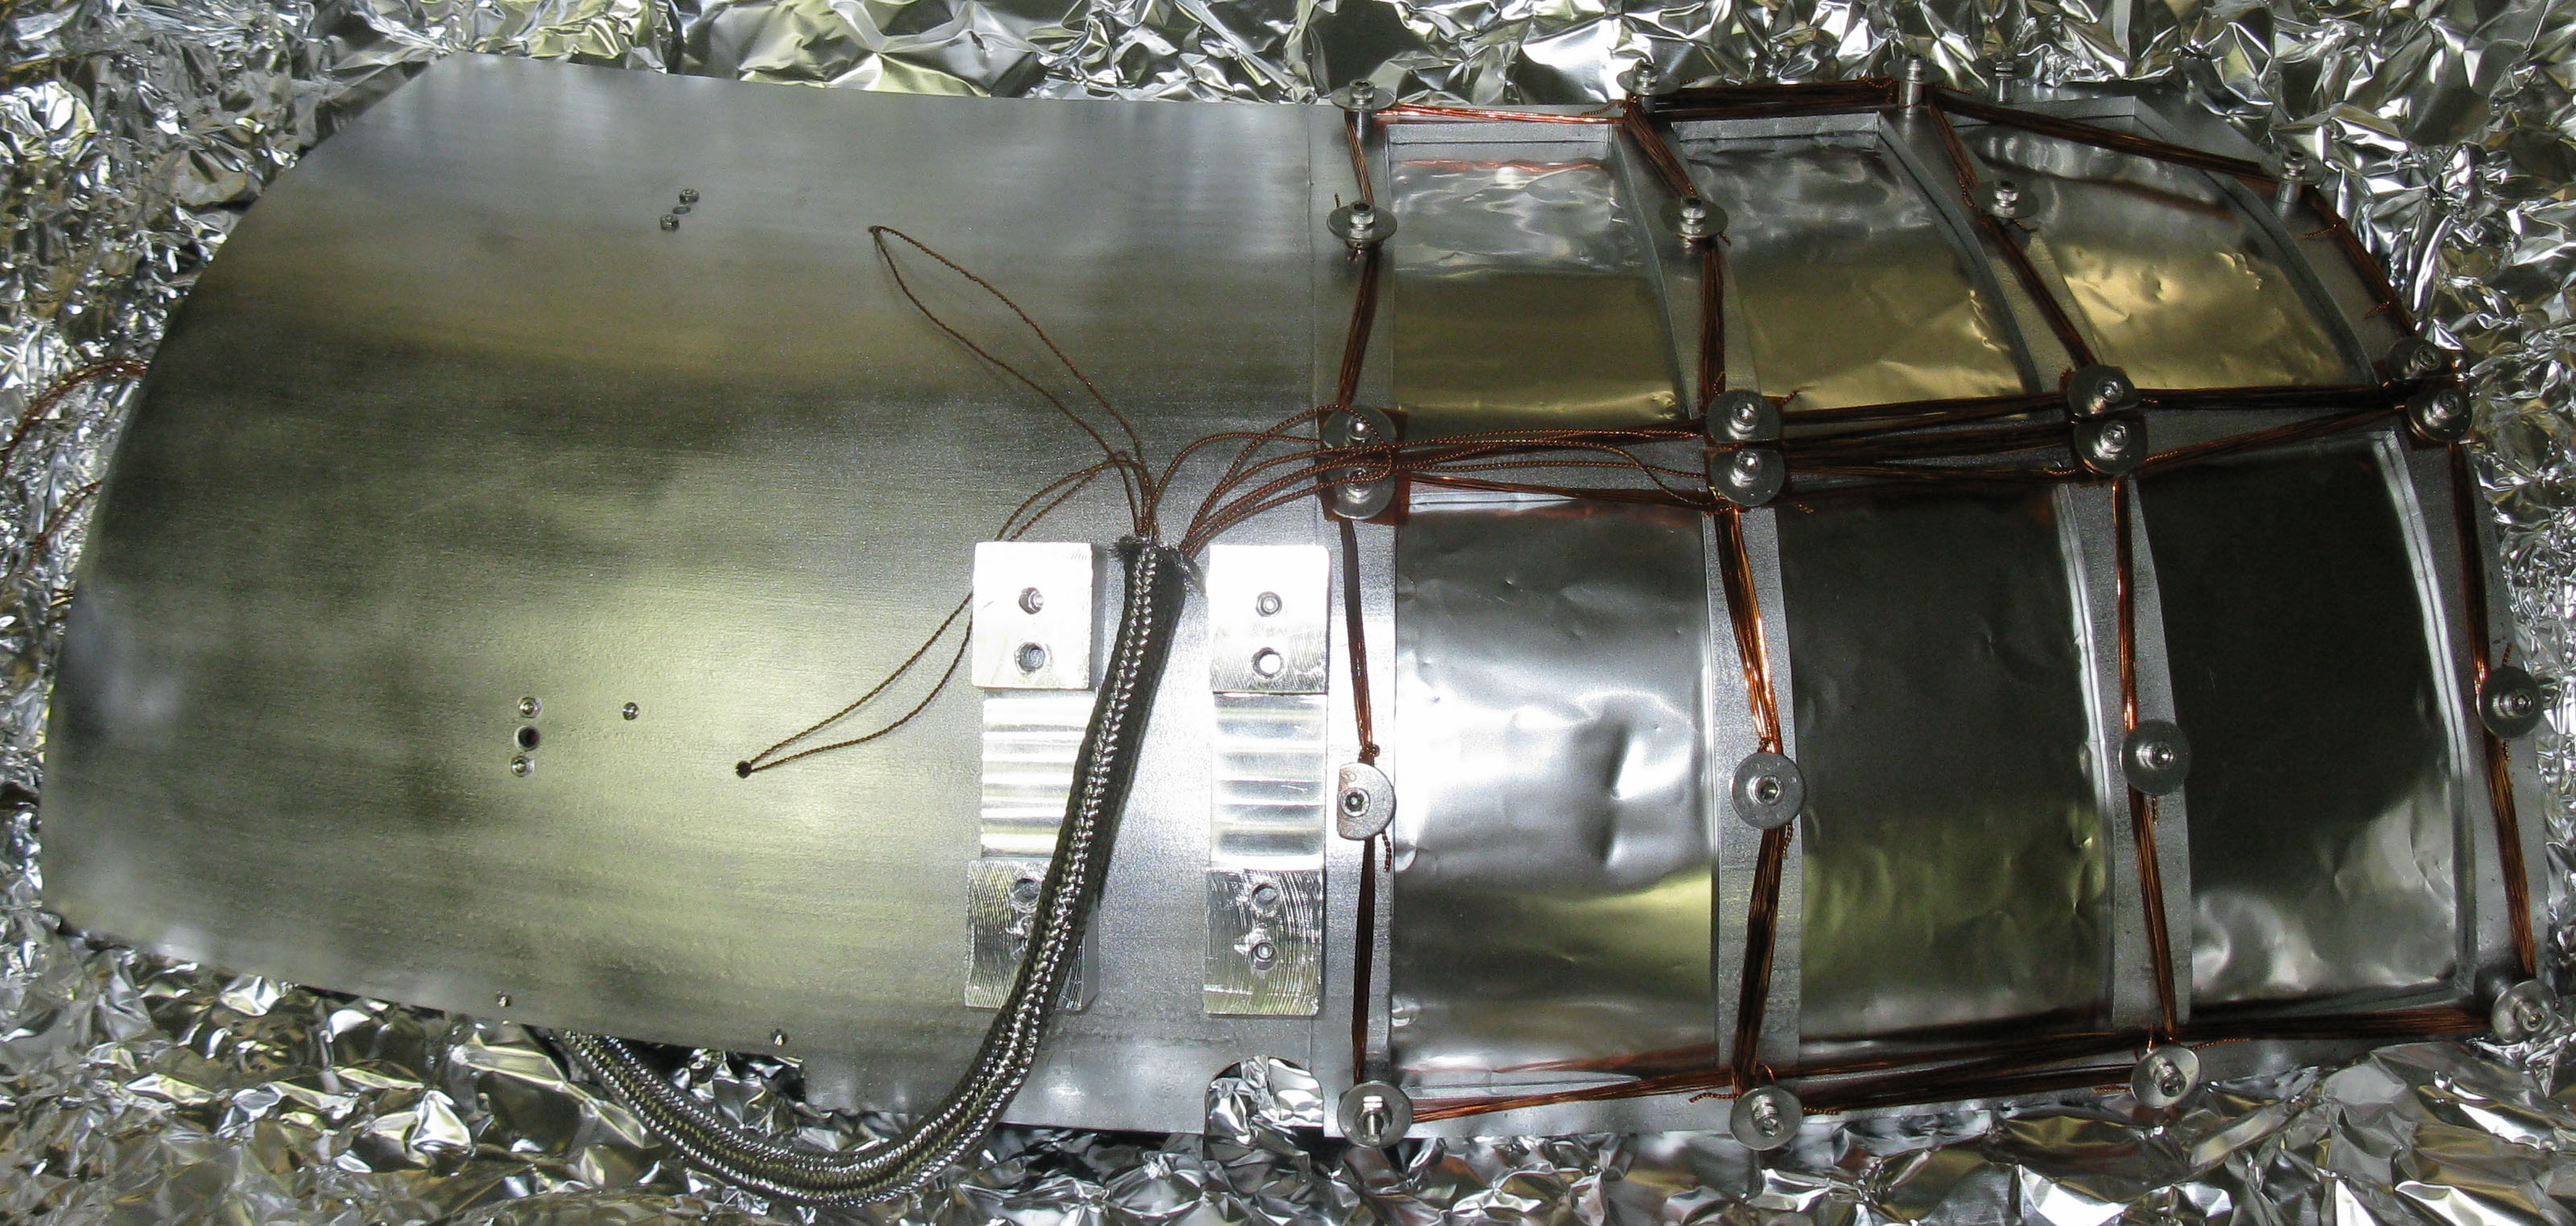
\includegraphics[width=0.9\columnwidth]{control_shell}\\

\item Saddle coil pairs fired with opposite polarity create a discrete analog to the shaping coil.
\item Currents in the coils are $\frac{1}{200}$ of the shaping coil, but are 5 times closer to the plasma surface.
\item A static, up/down symmetric perturbation was applied at $\theta \approx \pm$ 45$^{\circ}$, which caused the plasma to become more triangular or square.
\item It may be possible to divert (single or double null) a low current plasma discharge.

%\includegraphics[width=0.45\columnwidth]{cc_down_APS_12}\includegraphics[width=0.45\columnwidth]{cc_up_APS_12}

%\item Preliminary runs have already found strong effects on the 3-1 kink mode.
%\begin{center}
%\includegraphics[width=0.9\columnwidth]{Unshaped_APS_2012}
%Unshaped plasma. 3/1 mode is established from 1.5ms onwards.\\
%Mode becomes external at 2.25ms without significant change in amplitude\\
%\vspace{2cm}
%\includegraphics[width=0.9\columnwidth]{Trishaped_APS_2012}
%Triangularly shaped plasma.  3/1 mode establishes at 2ms.  \\
%Mode damps as it crosses q of 3, amplitude remains low after crossing.\\
% After shaping is turned off at 4ms, mode begins growing\\
%\vspace{2cm}
%\includegraphics[width=0.9\columnwidth]{Sqshaped_APS_2012}
%Square shaped plasma, q crash is characteristic.\\
%3-1 mode is stronger above 3 than just below.\\
%3-1 mode strengthens once more at q $\approx$ 2.5\\
%\end{center}

\end{itemize}

\section{Future Work}

\section*{Construction/Installation}
\begin{itemize}
\item After completing the database search, it will be known if nominal positional stability plays a role in HBT-EP.
\item If so, a VF/OH discharge must be developed that maintains stability in the presence of shaping.

\item Either way, construction of the power supply can begin soon, and full completion of the coil is expected within a year.

\item More runs can be taken with saddle coil shaping to prepare for full shaping runs and to further understand the 3-1 mode's reaction to shaping

\section*{Coil Shaping}

\item Work is underway to improve the robustness of the TokaMac code to the flux surface geometry currently of a shaped plasma.  

\item This would allow us to simulate the MHD behavior of the plasma under shaping.

\item More runs can be taken with saddle coil shaping to increase the database and further understand the 3-1 mode's reaction to shaping.

\item Active control of the saddle coils allows a much broader range of pulse shapes, many of which are impossible with a capacitive power supply.  

\end{itemize}


\section{Summary}
\label{sec:summary}

\begin{itemize}
\item The shaping coil is easy to install and low cost but will allow access to an entirely different regime of MHD physics for HBT-EP.  
\item Low inductance construction ensures that it will not significantly alter the standard HBT-EP discharge in non-shaped plasmas
\item Saddle coilset has demonstrated MHD effects of low power quasi-axisymmetric shaping, is a much more flexible instrument than the shaping coil.  
\item The results of saddle coil shaping can inform and guide our research with the shaping coil, and provide interesting results in their own right.
\end{itemize}

\section{Acknowledgements}

This work was supported by DOE grant DE-FGO2-86ER53222.

\bibliography{literature.bib}

\end{multicols}
\end{document}

